\documentclass{article}
\usepackage[utf8]{inputenc}
\usepackage[spanish]{babel}
\usepackage{ifpdf}
\usepackage{hyperref}
\usepackage{subcaption}
\usepackage{graphicx}
\usepackage{caption}
\title{Equipos e Instalaciones Eléctricas Aeronáuticas}
\author{Leandro Marsó}
\date{2015}
\ifpdf
\hypersetup{
    pdfauthor={Leandro Marsó},
    pdftitle={Equipos e Instalaciones Eléctricas Aeronáuticas},
}
\fi

% Para cambiar los nombres por defecto:
% Babel traducía table como cuadro. Yo lo cambio para tabla:
\addto\indexspanish{%
  \renewcommand{\indexname}%
    {Programa de la materia}%
}

\begin{document}
\maketitle
\pagebreak
\tableofcontents
\pagebreak
	\section{Electrostática}
La electrostática es el análisis de fenómenos en que las partículas con carga eléctrica se encuentran en reposo. O por decirlo de otra forma, con fuentes y campos eléctricos que no varían su valor según pasa el tiempo.

	\subsection{Carga eléctrica}
A partir de una serie de experimentos sencillos, Benjamín Franklin (1706-1790) determinó que existen dos tipos de cargas eléctricas, a las que dio el nombre de positiva y negativa. Los electrones tienen carga negativa y los protones positiva. Para comprobar la
existencia de ambos tipos de carga, realizamos el experimento Nº 1.

La unidad de carga más pequeña e conocida en la naturaleza, es la carga de un electrón (-e) o de un protón (+e), con una magnitud de
$$ e = 1,602 18 \times 10^{19} C$$

\subsubsection*{Experimento Nº 1}
Tomamos una cinta de teflón de aproximadamente 40cm y la sostenemos por la mitad. Notamos que la cinta cae libremente, con sus dos extremos muy cerca el uno del otro. Luego frótela varias veces con un material de lana, hasta ver que ambos extremos ya no se tocan mas al colgar, e incluso se separan formando una \textbf{v} invertida. Si luego acercamos a la cinta de teflón el mismo material de lana que utilizamos para frotar, observaremos que la cinta se eleva atraída por la lana. Esta observación demuestra que la cinta de teflón y la lana tienen dos tipos diferentes de carga. Con base en estas observaciones, se puede concluir que \textbf{cargas de un mismo signo se repelen y cargas de signos opuestos se atraen}.

	\subsection{Leyes y reglas de la electrostática}
	\subsubsection*{Ley de Coulomb}
En el siglo XVIII, el físico e ingeniero Charles Coulomb propuso un experimento que le permitió precisar las siguientes cuatro observaciones:

\begin{itemize}
\item Los cuerpos cargados sufren una fuerza de atracción o repulsión al aproximarse.
\item El valor de dicha fuerza es proporcional al producto del valor de sus cargas.
\item La fuerza es de atracción si las cargas son de signo opuesto y de repulsión si son del mismo signo.
\item La fuerza es inversamente proporcional al cuadrado de la distancia que los separa.
\end{itemize}

Coulomb determinó el valor de la fuerza que existe entre dos partículas cargadas como se muestra en la figura \ref{fig:cargasneg}:

\begin{center}
	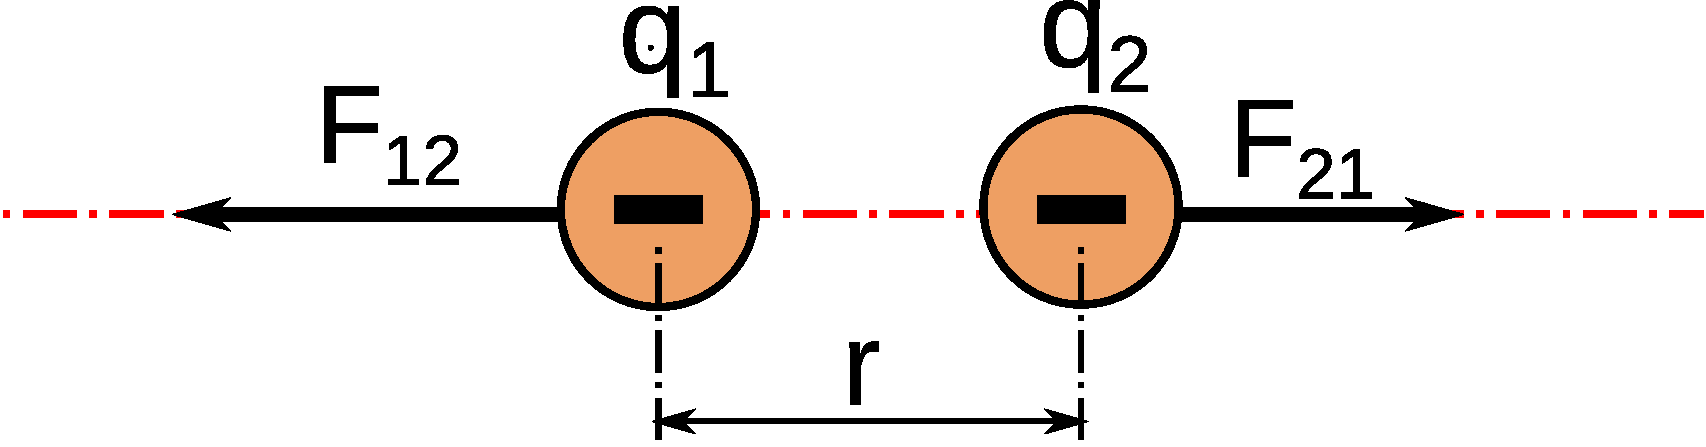
\includegraphics[scale=0.25]{figuras/cargasneg.pdf}
	\captionof{figure}{\emph{Dos partículas con carga eléctrica experimentan una fuerza debido a la existencia de la otra. Coulomb con su experimento, determinó las magnitudes de estas fuerzas}.}
\label{fig:cargasneg}
\end{center}

Coulomb sintetizó los resultados de su experimento con la siguiente ecuación:

\begin{equation}
|\vec{F}_{12}| = |\vec{F}_{21}| = \frac{q_1q_2}{r^2}k
\label{eq:CoulombForce}
\end{equation}


Donde $k$ es una constante conocida como \textbf{constante de Coulomb}. El valor de la constante de Coulomb depende del medio en que se encuentren las partículas (vacío, aire, agua, etc) y de la elección de las unidades. La unidad de carga del Sistema Internacional (SI) es el \textbf{coulomb} (C). La constante de Coulomb para el vacío (la nombramos como $k_e$) en unidades del SI tiene el valor
$$k_e = 8,9876 \times 10^9 N \cdot m^2/C^2$$

Además, esta constante se expresa como

$$k_e = \frac{1}{4\pi\epsilon_0} $$ 

donde $\epsilon_0$ (letra griega minúscula epsilon) es el valor de la permitividad del vacío.

Generalizando, decimos que $\epsilon = \epsilon_0\epsilon_r$, y $\epsilon_r$ es la permitividad dialéctrica relativa del medio en que se encuentren. Por ejemplo el $\epsilon_r$ del vacío es $1$, el de la mica es de $5,4$ y el del papel aprimadamente $50$. 

Volviendo a la ecuación \ref{eq:CoulombForce}, explicamos que 

\begin{itemize}
\item $\vec{F}_{12}$ es la fuerza sobre la carga $q_1$ debido a la existencia de la carga $q_2$, y $\vec{F}_{21}$ es la fuerza que  sobre la carga $q_2$ debido a la existencia de $q_1$. Esta fuerza en S.I. se mide en Newtons
\item $q_1$ y $q_2$ son los valores de dos cargas puntuales, en el S.I. se mide en Coulomb
\item $r$ es la separación entre las cargas, en metros para el S.I.
\item Como ya dijimos, $\epsilon$ es la constante de permitividad dialéctrica del medio en que se encuentran, para el vacío se denomina como $\epsilon_0$ y su valor es $8,85418 \times 10^{-12}$ Faradios/metro (F/m)
\end{itemize}

%	\subsection{Fenómenos electrostáticos}
	\subsection{Campo eléctrico}
El concepto de campo lo desarrolló Michael Faraday (1791-1867) en relación con las fuerzas eléctricas. Faraday planteó que existe un campo eléctrico en la región del espacio que rodea a un objeto con carga: la carga fuente. Cuando otro objeto con carga —la carga de prueba— entra en este campo eléctrico, una fuerza eléctrica actúa sobre él. 

Para ejemplificar, observe la figura \ref{fig:campo}, que muestra una pequeña carga de prueba positiva $q_0$ colocada cerca de un segundo objeto con una carga positiva $Q$ mucho mayor. El campo eléctrico provocado por la carga fuente en la carga de prueba es la fuerza eléctrica que actúa sobre la carga de prueba, dividida por el valor $q_0$:
$$
\vec{E}\equiv \frac{\vec{F}_e}{q_0}
$$

\begin{center}
	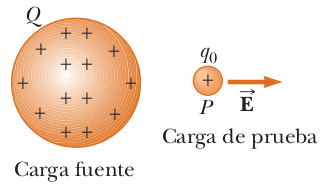
\includegraphics[scale=0.50]{figuras/campo-1.png}
	\captionof{figure}{\emph{Una pequeña carga de prueba positiva $q_0$ colocada en el punto P cerca de un objeto con una carga positiva $Q$ mucho mayor experimenta un campo eléctrico E en el punto P establecido por la carga fuente $Q$.}}
\label{fig:campo}
\end{center}

El vector $\vec{E}$ en unidades S.I. es: newtons por coulomb (N/C). Observe que $\vec{E}$ es el campo producido por una carga o distribución de carga separada de la carga de prueba; no es el campo producido por la propia carga de prueba, además observe que la existencia de un campo eléctrico es una propiedad de su fuente; la presencia de una carga de prueba no es necesaria para que el campo exista. La carga de prueba sirve como detector del campo eléctrico. La dirección de $\vec{E}$, como se muestra en la figura \ref{fig:campo}, es la dirección de la fuerza que experimenta una carga de prueba positiva cuando es colocada en el campo; \textbf{existe un campo eléctrico en un punto si una carga de prueba en dicho punto experimenta una fuerza eléctrica}.

\pagebreak


	\subsection{Inducción y líneas de fuerza}
	\subsection{Trabajo y energía eléctrica}
	\subsection{Diferencia de potencial}
	\subsection{Capacitores}

\section{Corriente Eléctrica}
\section{Magnetismo}
\section{Mediciones}
\section{Fuentes de alimentación}
\section{Distribución de la energía}
\section{Dispositivos de control de circuitos}
\section{Dispositivos de protección}
\end{document}
